\documentclass[12pt, a4paper]{report}

\usepackage[frenchb]{babel}
\usepackage[utf8]{inputenc}
\usepackage[T1]{fontenc}
\usepackage{eurosym}
\usepackage{fancyhdr}
\usepackage{xcolor}
\usepackage{graphicx}
\usepackage{here}
\usepackage{listings} 
\usepackage[colorlinks=true, pdfstartview=FitV, linkcolor=black, citecolor=blue, urlcolor=blue]{hyperref}
      
\definecolor{blue}{rgb}{0.13,0.29,0.46}
\definecolor{couleur_nom}{HTML}{336633}


\title{Mirage} 
\author{Illusion Corportation}
\date{}


\begin{document}
\thispagestyle{empty}
\begin{center}
\fontsize{16}{20pt}
\textbf{Mirage - Rapport de soutenance}
\end{center}
\vspace*{1.9cm}


\begin{figure}[!h]
\begin{center} 
\includegraphics[width=1.3\textwidth]{images/mirage_logo.png} \end{center}
\end{figure}

\vspace*{7.8cm}
\par
\begin{flushleft}
\fontsize{16}{21pt}
Youcef \textsc{El Kamel}
(\emph{el-kam\_y})
\newline
Salah \textsc{Aldemaski}
(\emph{aldema\_a})
\newline
William \textsc{De Michiel}
(\emph{de-mi\_w})
\newline
Chahine \textsc{Mouhamad}
(\emph{Mouha\_c})

\end{flushleft}


\newpage


\tableofcontents


\chapter{Rapport de soutenance final}


Mirage est un projet scolaire de seconde ann\'ee de l'\'ecole EPITA. Ce projet est d\' evelopp\'e par 4 \' etudiants d'INFO-SPE \`a partir de Janvier 2012 jusqu'\`a fin mai 2012. 
\par Nous sommes en deuxi\`eme ann\' ee (InfoSpe) \`a EPITA et ce projet informatique constitue notre troisieme r\' ealisation importante en groupe, apr\`es celle de cartographie realiser au premier semestre. 
\par Pour ce semestre, nous devons proposer un projet avec un algorithme plus complexe que nos deux derniers projet mais il nous faut évidemment  un projet qui nous intéresserait, On a donc choisi de faire un logiciel de retouche, de traitement et de dessin assisté par ordinateur.
\par Le nom de ce projet nous est venu des mirages que l'on peut voir dans le désert, en effet l'utilisateur grâce à notre logiciel pourra faire des créations tellement belle qu'il n'en croira pas ces yeux

\par le projet a etais finaliser avec succes. il est disponible sur internet et permet de faire de bonne creation.
\par nous avons finalement respecté le cahier des charges. 

\newpage


\chapter{Un groupe}

Comme vous le savez surement (ou pas), l'\'equipe Illusion Corporation est form\' e de Youcef Elkamel, Salah Aldemachki, William De Michiel et enfin de Chahine Mouhamad. 


\section{Youcef El Kamel}

\begin{figure}[!h]
\begin{center} 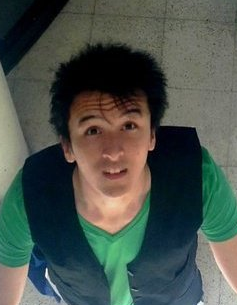
\includegraphics[width=0.5\textwidth]{images/youcef.png} \end{center}
\end{figure}

\par J’utilise Photoshop depuis déjà plusieurs années et cette fois-ci ayant un projet libre avec de bonne base en informatique, j’aimerai pouvoir faire un logiciel de traitement d’image et de création d’image. Heureusement, j’ai trouvé un groupe de personne ayant la même idée et motiver.
\par En tant que chef de projet, je mettrai un point d’honneur afin que le projet soit bien abouti et réaliser convenablement.
\par Je vais principalement m’occuper de tout ceux que l’utilisateur voit et utilise c’est-à-dire l’interface graphique et le site web mais ce n’est pas pour autant que je ne vais pas aider mes collègues pour concevoir certain algorithme de traitement d’image qui peuvent avoir une complexité algorithmique importante.


\newpage

\section{William De Michiel}

je suis quelqu'un de très créatif, j'aime crée et concevoir de nouvelles choses, et j'espère pouvoir donner un aboutissement à toutes mes idées concernant ce projet Mirage, afin de mettre en oeuvre des outils n'ayant pas étés déjà vus au paravent, dans un logiciel similaire à celui-là. Je souhaite ainsi pouvoir, a travers ce projet, améliorer mon niveau de programmation, acquérir de nouvelles connaissances, et en particulier, acquérir une première expérience avec le langage C dont je ne suis pas encore tres familier.

\begin{figure}[!h]
\begin{center} 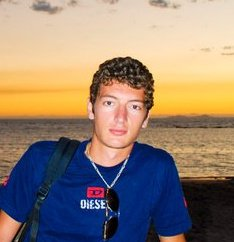
\includegraphics[width=0.5\textwidth]{images/wili.jpg} \end{center}
\end{figure}

\newpage

\section{Salah Aldemaskil}

Etudiant à Epita ce 3eme projet va me permettre d’apprendre un tout nouveau langage qui sera le C. Ce projet me permettra de m’améliorer une fois de plus au niveau du code mais aussi m’apprendre comment fonctionne les logiciels tels que Photoshop, Gimp et leur fonctionnalité. 
\par Mais aussi savoir que dans ce logiciel il a une part d’algorithme importante qu’on ne voit pas lorsque que l’on utilise ce logiciel. C’est pour cela que j’attends avec impatience ce projet.

\begin{figure}[!h]
\begin{center} 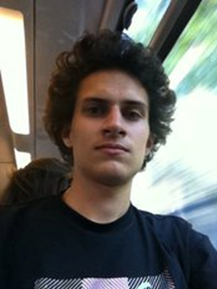
\includegraphics[width=0.5\textwidth]{images/sallah.png} \end{center}
\end{figure}


\newpage



\section{Chahine Mouhamad}

\par Nous allons utiliser le langage C et le Caml pour le développement de ce projet. Ma présence à Epita au second semestre m’oblige à vous parler d’avantage de ce qui se rapporte à l’informatique qu’au reste de ma vie. Disons donc que ces début en C me paraissent assez prometteur notamment du fait que j’ai plus de facilités à manipuler le Cshare que le Caml. Après les durs labeurs pour apprendre à coder en Caml pour le projet du premier semestre, puis les durs labeurs et les monstrueuses difficultés avec ce langage avec le Mini-projet, nous avons enfin la possibilité de coder avec un vrai langage : le C ! Adieu CamL ! Ce projet est l’occasion pour moi de découvrir le travail d’équipe avec de nouvelles personnes et probablement d’autres approches que celles vues avec mon ancien groupe sur les jeux vidéo et en SPE sur le projet de cartographie.
     \par    La liberté de sujet de projet est aussi très intéressante car elle laisse place à l’imagination de chacun et évitera au maximum d’avoir des projets similaires. De plus, le fait que le langage a utilisé est un des langages les plus connus en programmation est très motivant. 
\par Ce projet s’avère encore une fois très enrichissant au point de vue humain et social mais aussi au point de vue programmation, avec ce nouveau langage (même si on doit toujours utilisé le Caml). L’expérience que ce projet nous apportera prend donc une part importante dans ma motivation. Notamment les réactions de notre groupe face aux difficultés posées et à terme l’accomplissement de celui ci. Je vais m’investir pleinement dans ce projet afin d’avoir un bon rendu et surtout un logiciel qui fonctionne (enfin j’espère !).

\newpage

\chapter{les haut et les bas du projet}




\newpage


\chapter{Outils utiliser}

Pour réaliser ce projet nous allons utiliser plusieurs outils qui sont pour la plus part imposé à nous mais essentiel pour un informaticien

\section {Fedora}

Fedora, anciennement Fedora Core, est une distribution GNU/Linux basée sur le système RPM, développée par le Projet Fedora et soutenue par la société Red Hat. Cette distribution se veut être un système d'exploitation complet et généraliste, composé uniquement de logiciels libres. Fedora dérive donc de la distribution Red Hat Linux, et est destinée à la remplacer pour les utilisateurs finaux (utilisation non commerciale). Le maintien de Fedora provient en grande partie de sa communauté d'utilisateurs. Bien que Red Hat emploie de nombreux développeurs pour Fedora, l'entreprise ne fournit pas d'assistance officielle pour les utilisateurs du grand public.

\section {Ocaml}

\par OCaml, anciennement connu sous le nom d'Objective Caml est l'implémentation la plus avancée du langage de programmation Caml, créé par Xavier Leroy, Jérôme Vouillon, Damien Doligez, Didier Rémy et leurs collaborateurs en 1996. Ce langage, de la famille des langages ML, est un projet open source dirigé et maintenu essentiellement par l'INRIA.

\par OCaml est le successeur de Caml Light, auquel il a ajouté entre autres une couche de programmation objet. L'acronyme CAML provient de Categorical Abstract Machine Language, un modèle de machine abstraite qui n'est cependant plus utilisé dans les versions récentes de OCaml.

\par Portable et performant, OCaml est utilisé dans des projets aussi divers que le logiciel de synchronisation de fichiers Unison, l'assistant de preuves formelles Coq. Les facilités de traitement symbolique du langage permettent le développement d'outils de vérification statique, comme le projet SLAM1 pour des pilotes Windows écrits par Microsoft, ou ASTRÉE pour certains systèmes embarqués des Airbus A380.

\newpage

\section {le langage C}
Le C est un langage de programmation impératif conçu pour la programmation système. Inventé au début des années 1970 avec UNIX, C est devenu un des langages les plus utilisés. De nombreux langages plus modernes comme C++, Java et PHP reprennent des aspects de C.

\section { HTLM5/CSS}
 \par  HTML (HyperText Markup Language) : il a fait son apparition dès 1991 lors du lancement du Web. Son rôle est de gérer et organiser le contenu. C'est donc en HTML que vous écrirez ce que vous souhaitez que la page affiche : du texte, des liens, des images... Vous direz par exemple : "Ceci est mon titre, ceci est mon menu, voici le texte principal de la page, voici une image à afficher, etc.".
 \par    CSS (Cascading Style Sheets, aussi appelées Feuilles de style) : le rôle du CSS est de gérer l'apparence de la page web (agencement, positionnement, décoration, couleur, taille du texte...). Ce langage est venu compléter le HTML en 1996.
\par Le HTML définit le contenu (comme vous pouvez le voir, c'est brut de décoffrage !). Le CSS permet, lui, d'arranger le contenu et de définir la présentation : couleur, image de fond, marges, taille du texte...

\newpage


\section {Simple DirectMedia Layer}

Simple DirectMedia Layer (SDL) est une bibliothèque très utilisée dans le monde de la création d'applications multimédias en deux dimensions comme les jeux vidéo, les démos graphiques, les émulateurs, etc. Sa simplicité, sa flexibilité, sa portabilité et surtout sa licence GNU LGPL contribuent à son grand succès. Elle est de plus considérée comme un outil suffisamment simple, et est souvent conseillée aux programmeurs débutants pour commencer dans le monde de la programmation multimédia.

\begin{figure}[!h]
\begin{center} 
\includegraphics[width=0.8\textwidth]{images/sdl.png} \end{center}
\end{figure}



\newpage


\section {GTK+}

GTK+  est un ensemble de bibliothèques logicielles, c'est-à-dire un ensemble de fonctions informatiques, permettant de réaliser des interfaces graphiques. Cette bibliothèque a été développée originellement pour les besoins du logiciel de traitement d'images GIMP. GTK+ est maintenant utilisé dans de nombreux projets, dont les environnements de bureau GNOME, Xfce et ROX.

\begin{figure}[!h]
\begin{center} 
\includegraphics[width=0.8\textwidth]{images/gtk.png} \end{center}
\end{figure}


\newpage


\chapter{l'avancement du projet}

Dans ce chapitre, nous allons presenter les differents avancement du projet.

\section {la premiere soutenance }

Au debut nous avions du mal a commencer, nous ne savions pas quoi utiliser quel librairie, quel langage pour quel partie du projet etc... Mais finalement apres mur reflexion nous avons pu nous mettre d'accod. 
Ensuite l'une des partie les plus dur a etais de repartir les taches, nous ne savions pas quoi donner et a quel personne... cela c'est fait plus au moin au hassard et voila .
Lors de la premiere soutenance, nous avions quelque filtre et traitement d'image, nous pouvions dessiner a l'aide de la souris sur une fenetre et nous avions un debut de site web.
Notre soutenance c'etais bien passer et nous etions content 


\begin{figure}[!h]
\begin{center} 
\includegraphics[width=0.8\textwidth]{images/goouni.png} \end{center}
\end{figure}


\newpage 


\section {la deuxieme soutenance}


Pour la deuxième soutenance, nous avions grandement avancée. 
Notre site web étais fini, nous pouvions faire plusieurs forme géométrique polygone et cercle. Il était aussi possible de faire des dégradés de différentes couleurs. Nous pouvions sélectionner les couleurs à l'aide d'une palette de couleurs  situé dans la boite à outils.


\begin{figure}[!h]
\begin{center} 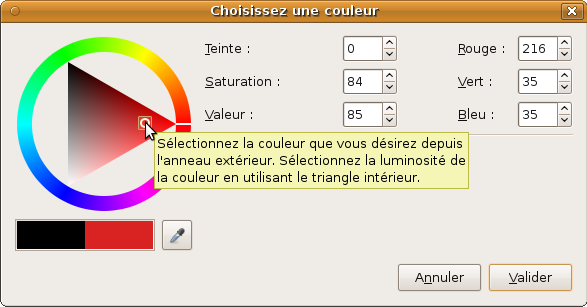
\includegraphics[width=0.8\textwidth]{images/palette.png} \end{center}
\end{figure}


\newpage







\chapter{Site Web}

\begin{figure}[!h]
\begin{center} 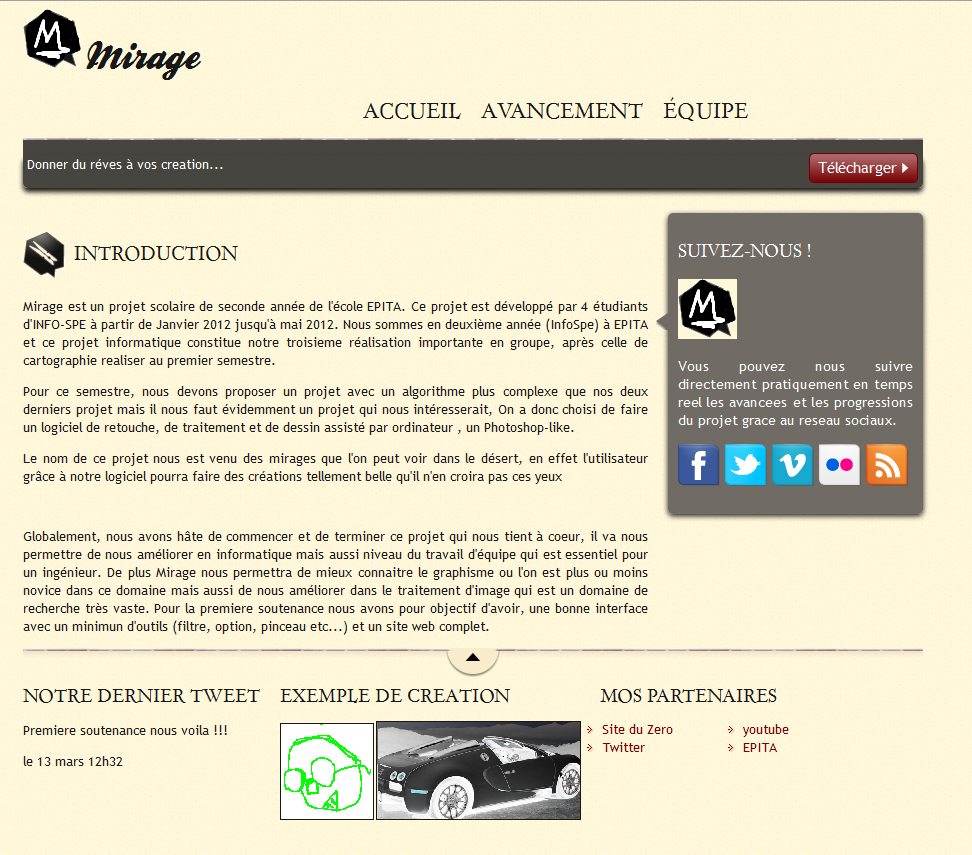
\includegraphics[width=0.8\textwidth]{images/site.png} \end{center}
\end{figure}

Notre site web ne se compose que de 3 grandes sections :

\par - L'accueil, ou le projet est présenté...

\par -  Equipe, une petite présentation des membres du groupes et quelque adresse pour nous contacter.

\newpage

\par - L'avancement, ou l'on poste tous les avancer du projet afin de bien montrer que nous avons respecté le cahier des charges qui est disponible en téléchargement a cette page.

\begin{figure}[!h]
\begin{center} 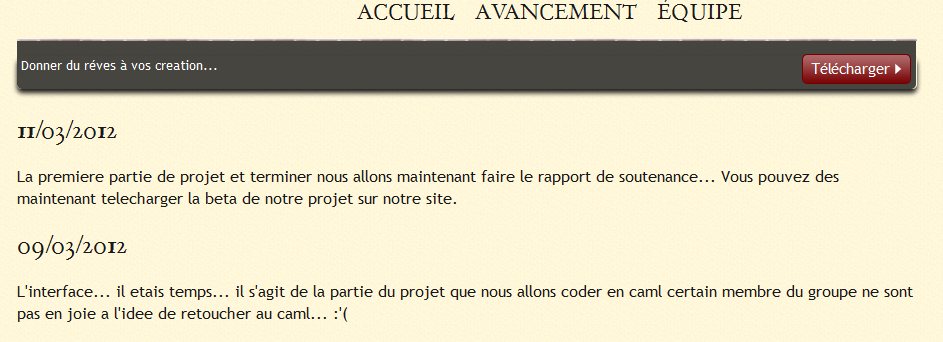
\includegraphics[width=1\textwidth]{images/avancement.png} \end{center}
\end{figure}


et l'on peut y telecharger l'executable du projet, il y a aussi la possibiliter de nous rejoindre dans plusieur reseau sociaux afin d'etre au courant de tout les mise a jours important et pour que les utilisateurs puissent nous prevenir d'eventuel bug.


\newpage





\chapter{Interface}


Nous avons développé une interface en Gtk en language C.
Grace a notre interface, on a la possibilité de charger et sauvegardé du texte et des images. 
Elle est composer de deux fenetre l'une est la boite a outils et l'autres la fenetre SDL.
l'utilisateur peut selectionner les couleurs et les outils dans la boite a outils et l'appliquer sur l'image. 

\section {La boite à outils}

Au début, il était possible de dessiner des formes seulement par le biais du manipulation clavier mais a force d’utiliser le programme,  nous nous sommes  rendu compte qu’il était très désagréable de passer de la souris au clavier et vice versa. De ce fait maintenant, tous se fait par le biais de la souris (sauf l’annulation et l’effacement de l’écran) : avec la boite a outils.

\begin{figure}[!h]
\begin{center} 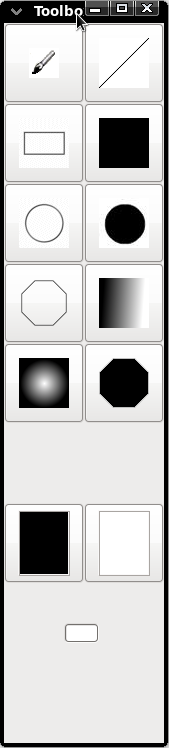
\includegraphics[width=0.2\textwidth]{images/outil.png} \end{center}
\end{figure}

\newpage 

Nous pouvons selectionner la couleurs que l'on veut a partir de la boite a outils, il y a toute les couleurs possible.



\begin{figure}[!h]
\begin{center} 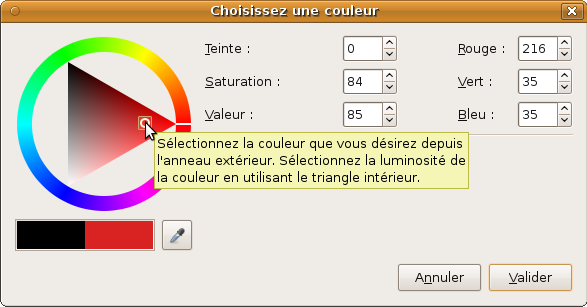
\includegraphics[width=0.5\textwidth]{images/palette.png} \end{center}
\end{figure}


\section {La fenetre SDL}

Cette fenetre n'est pas modulable  et est utiliser pour appliquer les outils selectionner avec la boite a outils

\begin{figure}[!h]
\begin{center} 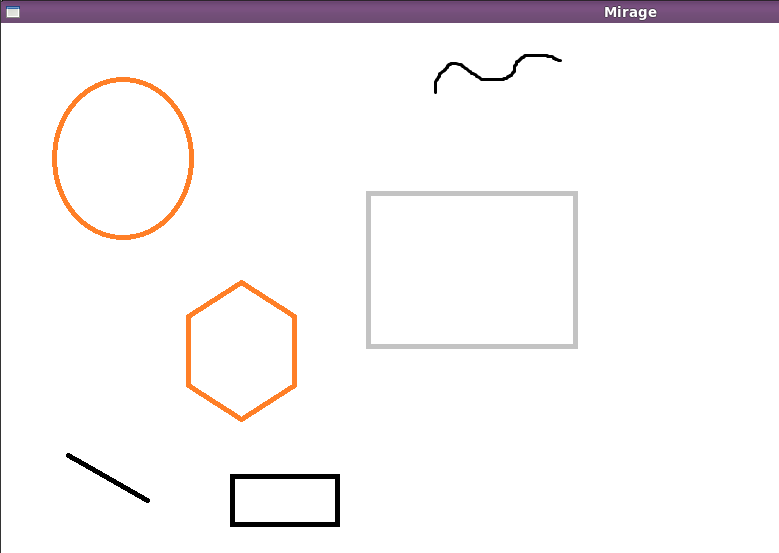
\includegraphics[width=0.7\textwidth]{images/inte.png} \end{center}
\end{figure}

Pour la dernière soutenance ils nous restent donc pour l’interface de pouvoir afficher les images, intégrer les filtres, le mode graphique qui nous permet de faire notre propre création et bien sur d’autre bonus ! 


\newpage

\chapter {les filtres}

\section {inverser les couleurs}

Nous pouvons desormais inverser les couleurs.
Cela a été assez simple à réaliser, il suffisait d'inverser les composante RGB.
Inverse les couleurs des pixel en prennant la couleur opposee (par exemple si une des composante d'un pixel est 255 elle devient egale a 0)

\begin{figure}[!h]
\begin{center} 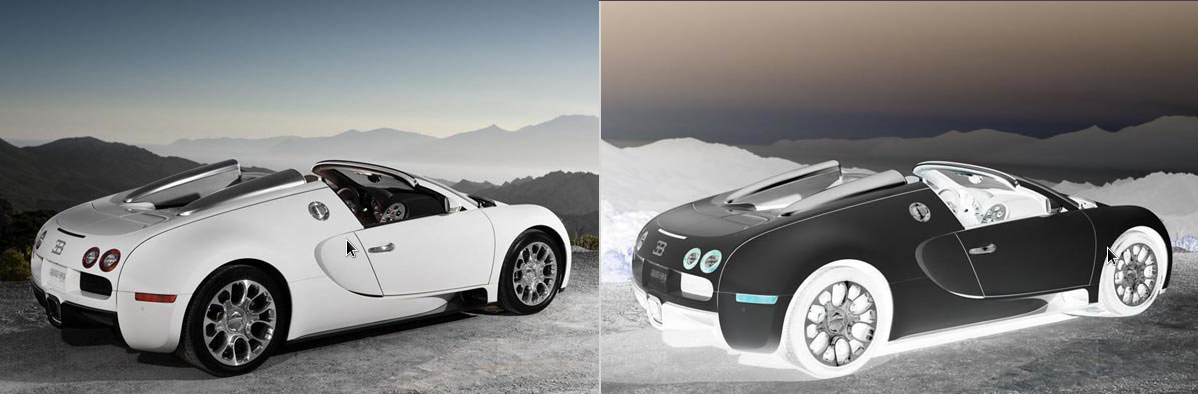
\includegraphics[width=1\textwidth]{images/inverse.png} \end{center}
\end{figure}

\newpage

\section{le floutage}

Nous pouvons appliquer un flou sur une image qui peut etre utile pour donner de l'importance a quelque chose de precis sur une image.
Les couleurs de deux pixels cote a cote son melanges donnant un effect de flou 

\begin{figure}[!h]
\begin{center} 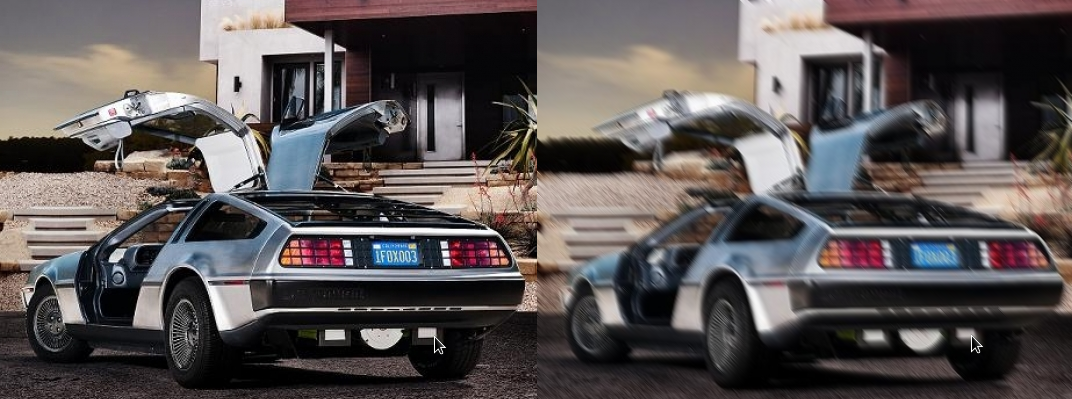
\includegraphics[width=1\textwidth]{images/flou.png} \end{center}
\end{figure}



\section{le mirroir}

Les pixels du cote gauche de l'image son recopies a droite faisant comme un mirroir verticale au mileu de l'image.
Pour les autres soutenance, nous essayerons de faire en sorte que l'utilisateur puissent choisir cette ligne de symetrie.


\begin{figure}[!h]
\begin{center} 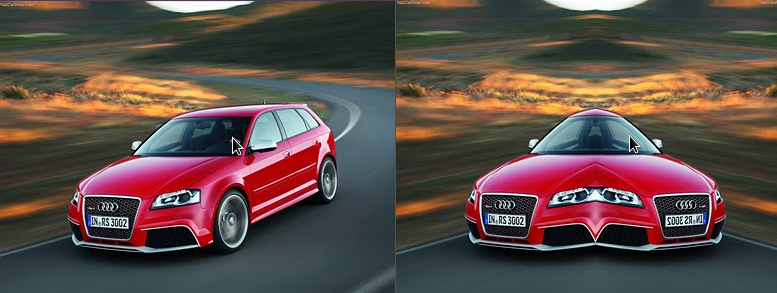
\includegraphics[width=1\textwidth]{images/mirroir.png} \end{center}
\end{figure}

\newpage

\section{la lumiere}

On peut modifier la lumiere en un point, les couleurs perdent plus ou moin de leurs intensite, et se ternissent jusqu a que l'image deviennent noir et blanc

\begin{figure}[!h]
\begin{center} 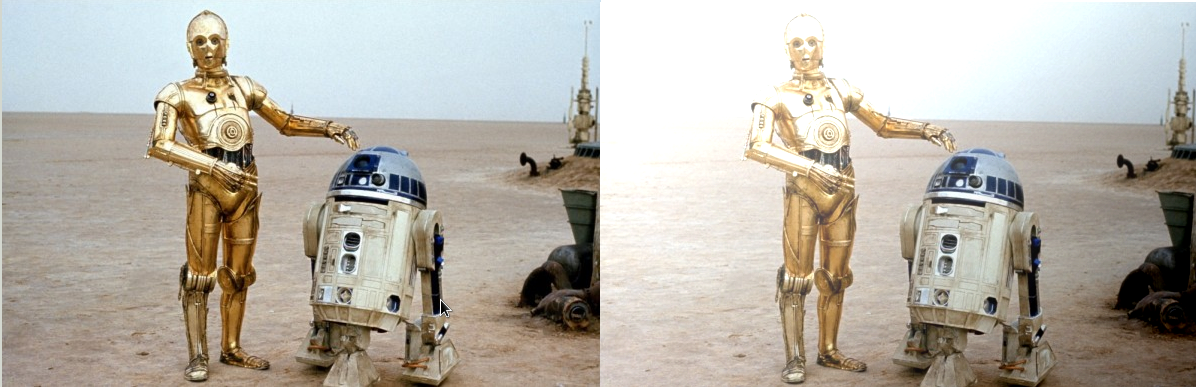
\includegraphics[width=1\textwidth]{images/lumi.png} \end{center}
\end{figure}



\section{le contraste}
suivant le contraste, les couleurs deviennent de plus en plus identiques(ou differente) entre elles.
l'on peut augmenter le contraste et les diminuiers.

\begin{figure}[!h]
\begin{center} 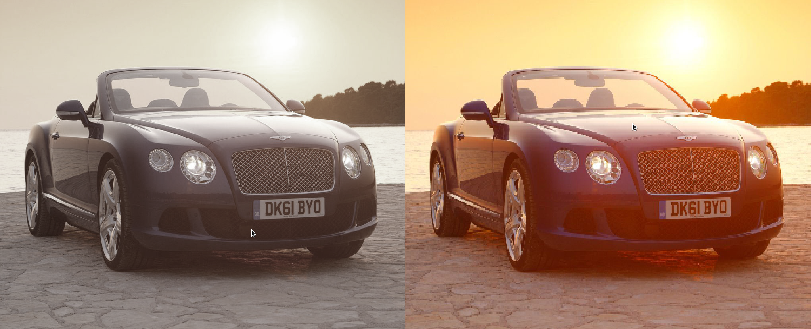
\includegraphics[width=1\textwidth]{images/foncer.png} \end{center}
\end{figure}

\newpage



\chapter {le dessin}


\par Tout d’abord, il la fallu qu’on choisisse une librairie afin d’écrire mes algorithme de trace de figures géométriques. 
\par Afin de ne pas nous compliquer la tâche, nous avons décidé d’opter pour SDL (Simple DirectMedia Layer) car il s’agit d’est une bibliothèque très utilisée dans le monde de la création d'applications multimédias en deux dimensions. 
\par Ensuite, nous avons dû décider quelles figures géométriques devaient être ajouté à notre éditeur d’images : pinceau, trait,  cercle, disque, rectangle (contours, plein), polygones (contours, plein), dégrade linéaire et dégrade circulaire.

\newpage


\section {le pinceau}

\begin{figure}[!h]
\begin{center} 
\includegraphics[width=0.5\textwidth]{images/drag.png} \end{center}
\end{figure}


L’outil pinceau est relativement facile à implémenter. En effet, il suffit de détecter un clic au niveau de la souris puis faire un “setpixel” aux coordonnées du clic. Pour la fonction “setpixel”, il a fallu qu’elle gère tous les formats (Uint8, Uint32,...) car je me suis rendu compte que cette fonction ne faisait pas la même chose selon le format du pixel de la surface que je manipule. Cependant, jusque-là mon outils pinceau avait un rayon égale a 1 (un seul pixel), mais pour faire varier sa taille j’ai du implémenter le trace du cercle plein par la suite.



\newpage

\section {les lignes }

\begin{figure}[!h]
\begin{center} 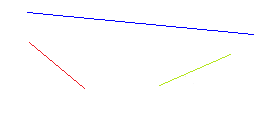
\includegraphics[width=0.8\textwidth]{images/line.png} \end{center}
\end{figure}

Il existe trois différents types de traits : vertical, horizontale et oblique. L’implémentation de lignes horizontales et verticales est très simple, ce qui n’est pas le cas pour les traits obliques. Apres quelques minutes de recherche sur internet, j’ai trouvé “l’algorithme de tracé de segment de Bresenham“. Cet algorithme permet de combler l’espace qu’il entre les points ou plus exactement : détermine quels sont les points d’un plan discret qui doivent être tracés afin de former une approximation de segment de droite entre deux points donnés.

\newpage

\section {les rectangles}

\begin{figure}[!h]
\begin{center} 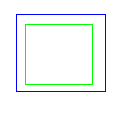
\includegraphics[width=0.8\textwidth]{images/carre.png} \end{center}
\end{figure}

Par rapport au rectangle, il existe deux types : creux ou plein. Pour les rectangles, il faut juste utiliser la methode SDLFillRect et le tour est joué. Enfin, pour les rectangles creux, on trace les quatre traits reliant chacun des quatre sommets formant le rectangle.

\newpage

\section {les cercles }

\begin{figure}[!h]
\begin{center} 
\includegraphics[width=0.8\textwidth]{images/cercle.png} \end{center}
\end{figure}

Comme pour les traits, j’avais un petit souci au niveau des extrémités des cercles selon l’axe horizontales. En effet, il manquait certains pixels de sortes que le cercle soit continu. Comme pour les traits il existe un algorithme spécialement fait pour : L’algorithme de tracé de cercle d'Andres : il permet, pour une complexité algorithmique très réduite, de tracer des cercles en image matricielle. Cet algorithme permet de paver entièrement le plan par des cercles concentriques, sans les trous.
Pour faire des cercles pleins, il suffit de relier les points symétriques en utilisant la fonction utilise pour faire des traits. En effet, cet algorithme trace le cercle octant par octant sachant les 7 derniers octants sont déduis par symétrie.


\newpage

\section {les polygones }


\begin{figure}[!h]
\begin{center} 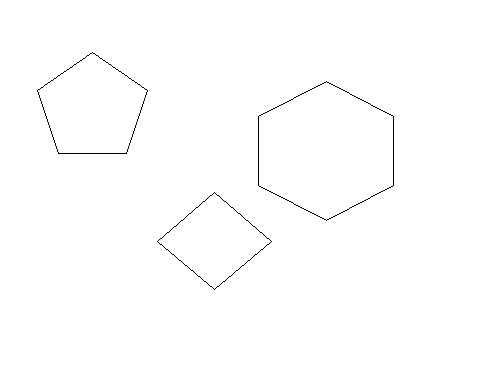
\includegraphics[width=0.8\textwidth]{images/poly.png} \end{center}
\end{figure}

Afin de trace un polygone, je me suis inspire de l’algorithme de trace de cercle. Pour tracer le polygone je dois d’abord déterminer la position de chaque sommet puis les ajouter dans une liste. Pour calculer la position des sommets j’utilise les propriétés trigonométriques : sin et cos. Une fois que la liste est construite, je la parcours en reliant les sommets deux a deux.


\newpage

\section {les degradés }



\begin{figure}[!h]
\begin{center} 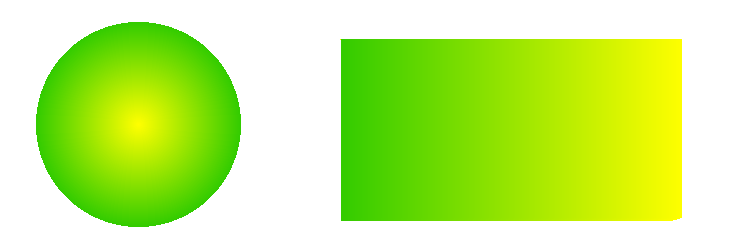
\includegraphics[width=1\textwidth]{images/degrader.png} \end{center}
\end{figure}


Pour faire un dégradé linéaire (dans un rectangle) je fais varier la couleur du premier seuil jusqu’a atteindre le second. Cependant je ne peux pas faire varier directement la couleur mais les composantes de la couleur. Enfin, pour tracer le rectangle j’utilise la fonction DrawLine utilise pour tracer des traits.
Pour les dégradés circulaires, j’utilise exactement la même méthode sauf que je fais varier le rayon lorsque je dessine un cercle.


\newpage

\section {Trace artistique}

\begin{figure}[!h]
\begin{center} 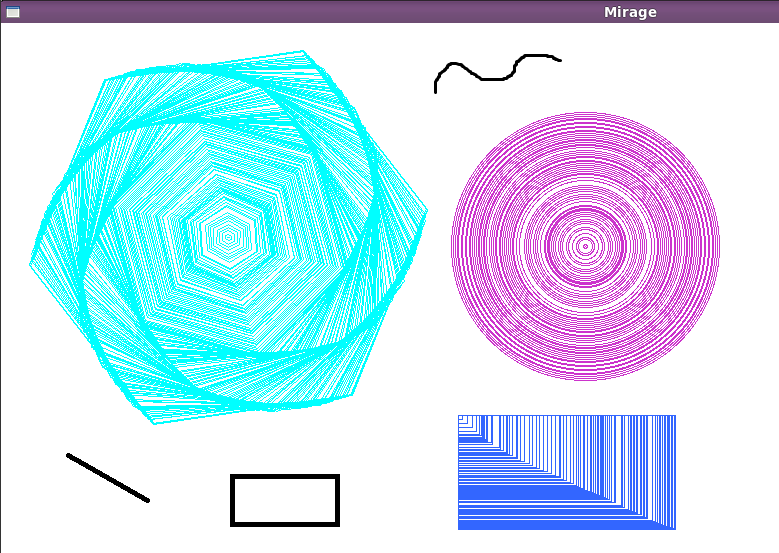
\includegraphics[width=1\textwidth]{images/tracebo.png} \end{center}
\end{figure}

Un des problèmes que je n’ai pas réussi à résoudre est lorsque je dessine un cercle, par exemple, je dessine tous les précèdent cercles que j’ai dessine lorsque l’appuie sur la souris était maintenue. Cependant, cela permet de créer de très belles formes. 


\newpage






\section {annulation de la derniere tache}


Afin d’améliorer l’expérience de l’utilisateur, la touche ‘Retour’ permet d’annuler la dernière modification. Pour cela j’enregistre l’état de l’image qui est affiche à chaque fois que l’utilisateur a fini d’utiliser un outil. Enfin, pour effacer l’écran, il suffit d’appuyer sur la touche ‘c’.

\section {Charger et sauvegarder l’image}


Le chargement et la sauvergarde de l’image se fait lorsqu’on execute le programme :

>./mirage input.jpg output.bmp par exemple

si l’utilisateur ne speficie aucun argument input.jpg sera une image blanche et les modifications seront enregistres sous le fichier output.bmp.

\begin{figure}[!h]
\begin{center} 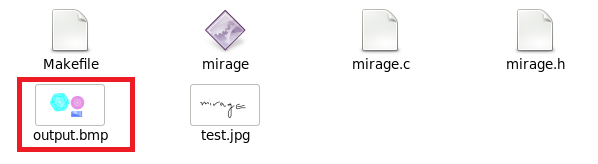
\includegraphics[width=1\textwidth]{images/sauve.png} \end{center}
\end{figure}


\newpage






\chapter{Conclusion}
\par Globalement nous avons bien progresser depuis la premiere soutenance, il ne nous reste plus qu'une derniere echeance. \par Nous esperons d'ici la pouvoir tout reunir c'est a dire les filtres, l'interface et la fenetre SDL ! ce qui d'apres se que nous avons vu ne sera pas une tache facile. 
Apres ceci, il ne nous reste plus qu'a faire plusieurs type de pinceau differrent et un historique visuel.

\end{document} 